%%%%%%%%%%%%%%%%%%% vorlage.tex %%%%%%%%%%%%%%%%%%%%%%%%%%%%%
%
% LaTeX-Vorlage zur Erstellung von Projekt-Dokumentationen
% im Fachbereich Informatik der Hochschule Trier
%
% Basis: Vorlage svmono des Springer Verlags
%
%%%%%%%%%%%%%%%%%%%%%%%%%%%%%%%%%%%%%%%%%%%%%%%%%%%%%%%%%%%%%

\documentclass[envcountsame,envcountchap, deutsch]{i-studis}

\usepackage{makeidx}         	% Index
\usepackage{multicol}        	% Zweispaltiger Index
%\usepackage[bottom]{footmisc}	% Erzeugung von Fußnoten

%%-----------------------------------------------------
%\newif\ifpdf
%\ifx\pdfoutput\undefined
%\pdffalse
%\else
%\pdfoutput=1
%\pdftrue
%\fi
%%--------------------------------------------------------
%\ifpdf
\usepackage[pdftex]{graphicx}
\usepackage{epstopdf}
\usepackage[pdftex,plainpages=false]{hyperref}
%\else
%\usepackage{graphicx}
%\usepackage[plainpages=false]{hyperref}
%\fi

%%-----------------------------------------------------
\usepackage{color}				% Farbverwaltung
%\usepackage{ngerman} 			% Neue deutsche Rechtsschreibung
\usepackage[english, ngerman]{babel}
%\usepackage[latin1]{inputenc} 	% Ermöglicht Umlaute-Darstellung
\usepackage[utf8]{inputenc}  	% Ermöglicht Umlaute-Darstellung unter Linux (je nach verwendetem Format)

%-----------------------------------------------------
\usepackage{listings} 			% Code-Darstellung
\lstset
{
	basicstyle=\scriptsize, 	% print whole listing small
	keywordstyle=\color{blue}\bfseries,
								% underlined bold black keywords
	identifierstyle=, 			% nothing happens
	commentstyle=\color{red}, 	% white comments
	stringstyle=\ttfamily, 		% typewriter type for strings
	showstringspaces=false, 	% no special string spaces
	framexleftmargin=7mm, 
	tabsize=3,
	showtabs=false,
	frame=single, 
	rulesepcolor=\color{blue},
	numbers=left,
	linewidth=146mm,
	xleftmargin=8mm
}
\usepackage{textcomp} 			% Celsius-Darstellung
\usepackage{amssymb,amsfonts,amstext,amsmath}	% Mathematische Symbole
\usepackage[german, ruled, vlined]{algorithm2e}
\usepackage[a4paper]{geometry} % Andere Formatierung
\usepackage{bibgerm}
\usepackage{array}
\hyphenation{Ele-men-tar-ob-jek-te  ab-ge-tas-tet Aus-wer-tung House-holder-Matrix Le-ast-Squa-res-Al-go-ri-th-men} 		% Weitere Silbentrennung bei Bedarf angeben
\setlength{\textheight}{1.1\textheight}
\pagestyle{myheadings} 			% Erzeugt selbstdefinierte Kopfzeile
\makeindex 						% Index-Erstellung

\usepackage[official]{eurosym}
\usepackage{graphicx}
\usepackage{wrapfig}
%\usepackage{amsthm}
\usepackage{amsfonts}
\usepackage[mathscr]{euscript}

%--------------------------------------------------------------------------
\begin{document}
%------------------------- Titelblatt -------------------------------------
\title{Exemplarische Implementierung des Lichtschnittverfahrens mittels einer selbstgebauten Scan-Vorrichtung}
%\subtitle{English Title}
%---- Die Art der Dokumentation kann hier ausgewählt werden---------------
%\project{Bachelor-Projektarbeit}
%\project{Bachelor-Abschlussarbeit}
\project{Master-Projektstudium}
%\project{Master-Abschlussarbeit}
%\project{Seminar zur Vorlesung ...}
%\project{Hausarbeit zur Vorlesung ...}
%--------------------------------------------------------------------------
\supervisor{Professor Dr. Jürgen Lohscheller} 		% Betreuer der Arbeit
\author{David Wichter} 							% Autor der Arbeit
\address{Trier,} 							% Im Zusammenhang mit dem Datum wird hinter dem Ort ein Komma angegeben
\submitdate{Abgabedatum} 				% Abgabedatum
%\begingroup
%  \renewcommand{\thepage}{title}
%  \mytitlepage
%  \newpage
%\endgroup
\begingroup
  \renewcommand{\thepage}{Titel}
  \mytitlepage
  \newpage
\endgroup
%--------------------------------------------------------------------------
\frontmatter 
%--------------------------------------------------------------------------
%\input{chapters/Vorwort}				% Vorwort (optional)
\kurzfassung

%% deutsch
\paragraph*{}
In der Kurzfassung soll in kurzer und prägnanter Weise der wesentliche Inhalt der Arbeit beschrieben werden. Dazu zählen vor allem eine kurze Aufgabenbeschreibung, der Lösungsansatz sowie die wesentlichen Ergebnisse der Arbeit. Ein häufiger Fehler für die Kurzfassung ist, dass lediglich die Aufgabenbeschreibung (d.h. das Problem) in Kurzform vorgelegt wird. Die Kurzfassung soll aber die gesamte Arbeit widerspiegeln. Deshalb sind vor allem die erzielten Ergebnisse darzustellen. Die Kurzfassung soll etwa eine halbe bis ganze DIN-A4-Seite umfassen.

Hinweis: Schreiben Sie die Kurzfassung am Ende der Arbeit, denn eventuell ist Ihnen beim Schreiben erst vollends klar geworden, was das Wesentliche der Arbeit ist bzw. welche Schwerpunkte Sie bei der Arbeit gesetzt haben. Andernfalls laufen Sie Gefahr, dass die Kurzfassung nicht zum Rest der Arbeit passt.

%% englisch
\paragraph*{}
The same in english.
 			% Kurzfassung Deutsch/English
\tableofcontents 						% Inhaltsverzeichnis
\listoffigures 							% Abbildungsverzeichnis (optional)
%\listoftables 							% Tabellenverzeichnis (optional)
%--------------------------------------------------------------------------
\mainmatter                        		% Hauptteil (ab hier arab. Seitenzahlen)
%--------------------------------------------------------------------------
% Die Kapitel werden in separaten .tex-Dateien abgelegt und hier eingebunden.
\chapter{Einleitung}
\label{chap:Einleitung}
In allen sich mit Phänomenen und Gegenständen der erfahrbaren Außenwelt beschäftigenden Bereichen von Wissenschaft und Industrie ist das Vermessen eben jener Gegenstände von höchstem Interesse. Die Messtechnik als Schnittstelle zwischen der empirischen und der mathematisch-quantifizierten Welt ermöglicht erst als solche das Aufstellen und Validieren von Modellen, welche erfahrene Realitäten abbilden sollen. Es überrascht also nicht, dass gerade im Zuge von technologischem Fortschritt auch immer neue Methoden und Möglichkeiten gesucht werden, Objekte von Interesse zu vermessen. \newline
Eine dieser (realtiv) neuen Methoden besteht in dem Abtasten von Objekten mittels eines Lasers. Dieses Verfahren wurde zuerst in den 60er Jahren erfolgreich eingesetzt, auch wenn die ersten industriellen Anwendungen noch ca. 20 Jahre auf sich warten ließen (vgl. \cite{Ebrahim:11}). Dabei wird ein Laser auf ein zu vermessendes Objekt projiziert und mittels der räumlichen Informationen, die über den Laseremitter an sich, die Laserprojektion oder den Blickwinkel des Betrachters der Projektion bekannt sind, wird eine Distanzvermessung vorgenommen. Welche dieser Informationen wie verarbeitet wird, hängt von dem eingesetzten Verfahren ab. Bei den meisten Verfahren werden aus genügend gesammelten Distanzen dann 3D-Modelle des zu vermessenden Objektes angefertigt. Man spricht dann von einem 3D-Laserscanning. \newline
Industrielle Laserscanner werden heutzutage in vielen Bereichen der Vermessungstechnik benutzt und sind von der Minenvermessung (vgl. \cite{riegl:17}) bis zur Forensik (vgl. \cite{Zoller:16}) in allen möglichen Anwendungsbereichen vertreten. Diese Scanner weisen eine hohe Genauigkeit auf, sind für Privatpersonen meistens jedoch zu teuer. Da jedoch auch die Funktionsweisen von professionellen Laserscannern fundamentalen Prinzipien folgen, sind die an sich eingesetzten Verfahren vergleichsweise leicht nachzuvollziehen. Daher wurde für die vorliegende Ausarbeitung der Versuch unternommen, einen "`Do It Yourself''-Laserscanner zu bauen. Dieser soll das Lichtschnittverfahren als eine konkrete Art des Laserscannings erfolgreich mit Hilfe von Matlab als Entwicklungsumgebung umsetzen. In der Implementierung ist die Konstruktion einer Scan-Vorrichtung, die zugehörige Software und das Durchführen des Vermessungsverfahrens an sich enthalten. Es wurde vor allem auf die Einhaltung folgender Design-Prinzipien geachtet:
\begin{description}
\item[Simplizität] \hfill \\
Der Scanner sollte einfach zu konstruieren und zu bedienen sein. Außerdem sollten sich sowohl die Berechnungen als auch die Software, in der besagte Berechnungen stattfinden, leicht nachvollziehen lassen. Dies macht den Umgang mit dem Scanner komfortabler und begünstigt Nachbauten.
\item[Bezahlbarkeit] \hfill \\		
Der Scanner sollte preisgünstig konstruierbar sein und auch ohne High-End-Komponenten akzeptable Ergebnisse liefern.  
\item[Genauigkeit] \hfill \\  		
Ohne genaue Ergebnisse ist das Unterfangen einer Vermessung unnütz. Daher muss der Laserscanner unter der Annahme einiger Randbedingung möglichst genaue und reproduzierbare Messergebnisse liefern, welche das gemessene Objekt gebührend präzise als 3D-Modell abbilden.
\end{description}
In den folgenden Kapiteln wird zuerst auf die mathematische Theorie des Lichtschnittverfahrens eingegangen. Es folgt die konkrete Implementierung und die Beschreibung, wie der Scanner konstruiert wurde und wie bei einem einzelnen Scanvorgang die Vermessung und Datenverarbeitung durchgeführt wird. Anschließend werden die Ergebnisse begutachtet und es wird erläutert, wie erfolgreich die Hauptbearbeitungsschritte der Laserlinienerkennung und Koordinatenberechnung sind und warum. Geschlossen wird mit einem Fazit, welches alternative Techniken sowie mögliche weiterführende Schritte und Verbesserungen anführt.  

\begin{figure}
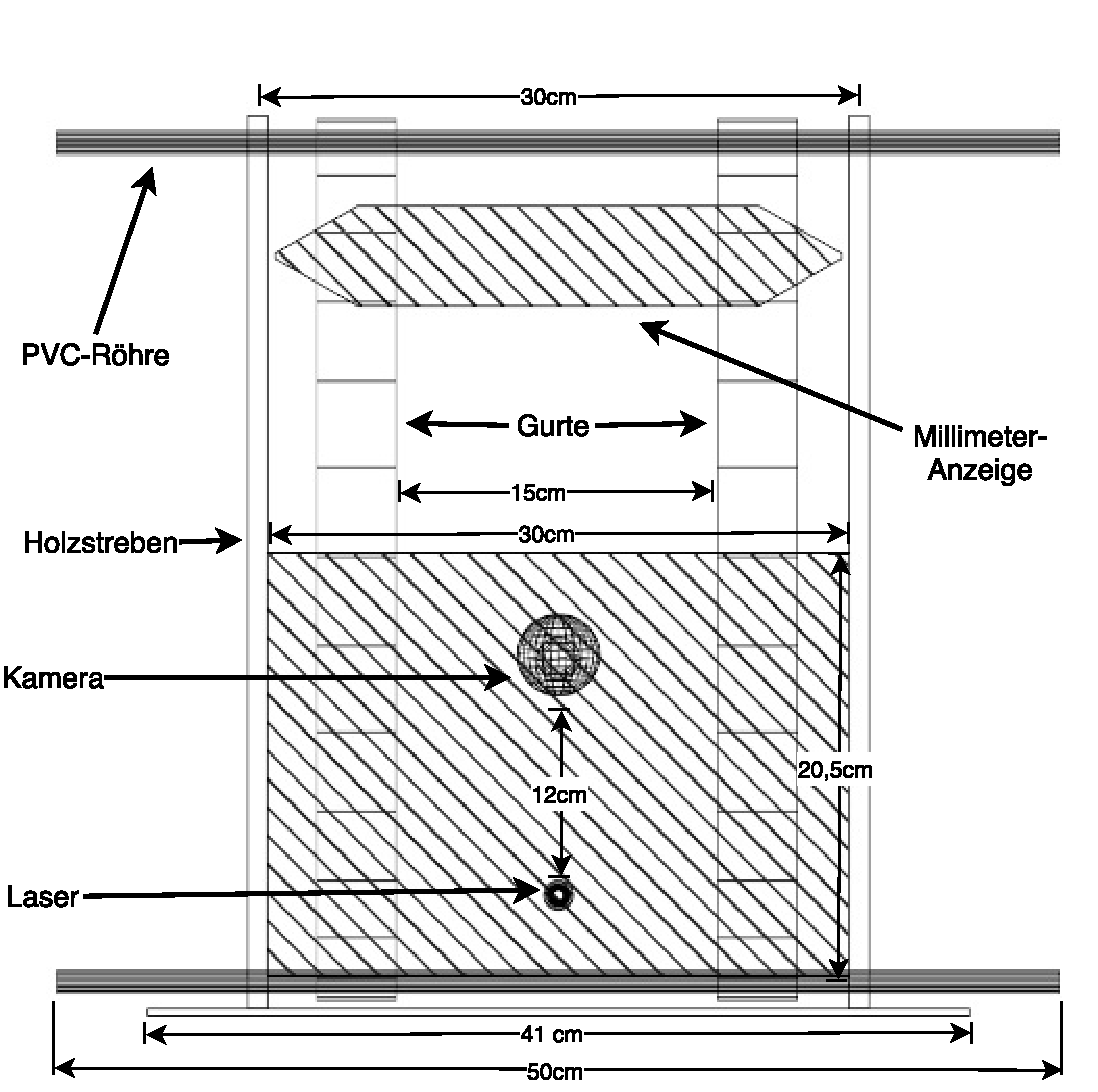
\includegraphics[width=\textwidth]{images/test.pdf}
\caption{Die Stufen des Scanvorgangs schematisch dargestellt}
\end{figure}


\chapter{Das Verfahren in der Theorie}
In diesem Kapitel wird auf die theoretischen Grundlagen des Verfahrens eingegangen. Es handelt sich dabei um eine Zusammenfassung, welche die wichtigsten Konzepte für das weitere Verständnis aufbereiten soll und beschränkt sich daher auf das Wesentliche. Weiterführende Lektüre, welche für die folgenden Abschnitte auch als Quelle gedient hat, ist unter anderem zu finden bei \cite{Simek:12}, \cite{Mathworks:17b} oder \cite{Rahmann}.

\section{Das mathematische Modell einer Kamera}
Das Lichtschnittverfahren macht sich nicht nur den eingangs erwähnten Laser zu Nutze, sondern nutzt zusätzlich eine Kamera um die räumlichen Informationen des vermessenen Objektes zu rekonstruieren. Die Kamera dient dabei als Betrachter der projizierten Laserlinie. Mathematisch wird hier das Modell einer Lochkamera zugrunde gelegt. Bei diesem Modell wird angenommen, dass Lichtstrahlen, die von einem Objekt reflektiert werden, durch den Fokuspunkt der Kamera fallen, dort gebündelt werden, und anschließend auf der anderen Seite des Fokuspunktes auf eine gegenüberliegende Projektionsfläche geworfen werden. So entsteht auf der Projektionsfläche das invertierte Bild des Objektes. Abb. \ref{fig:lochkamera} verdeutlicht das Modell. 

\begin{figure}
\centering \includegraphics{images/lochkamera.png}
\caption[Modell einer Lochkamera]{Modell einer Lochkamera. Quelle: \cite{Mathworks:17b}}\label{fig:lochkamera}
\end{figure}

Es handelt sich also um eine Projektion vom dreidimensionalen Raum, dem Weltkoordinatensystem, auf eine zweidimensionale Fläche, im Folgenden als Bildebene bezeichnet. Wie diese Projektion stattfindet, hängt vor allem von zwei Kamera-abhängigen Sets an Parametern ab: Den intrinsischen und den extrinsischen Kameraparametern. Erstere hängen lediglich von der Beschaffenheit der Kamera ab und ändern sich nicht wenn die Kamera ihre Position im Raum ändert. Hierunter fallen die Brennweite der Kamera ("`Focal length'' in der oben stehenden Abbildung) sowie der Ursprung des Bildebenenkoordinatensystms. Außerdem wird hierüber eine Scherung des projizierten Bildes bestimmt. Die intrinsischen Parameter können als 

\begin{equation}
K = \begin{pmatrix}
f_x & s & x_0 \\
0 & f_y & y_0 \\
0 & 0 & 1 
\end{pmatrix}
\end{equation}

 in einer Matrix zusammengefasst werden, in welcher \(f_x\) und \(f_y\) für die Brennweite in Pixeln (bei perfekt quadratischen Pixeln gilt \(f_x = f_y\)), \(s\) für die Scherung und \(y_0\) sowie \(x_0\) für die Verschiebung des Bildkoordinatenursprung in \(X\)- und \(Y\)-Richtung in Pixeln stehen. 
\newline
Im Gegensatz dazu definieren die extrinsischen Parameter die Orientierung und die Position der Kamera im Weltkoordinatensystem. Entsprechend werden diese als eine Rotationsmatrix \(R\) und ein Ortsvektor \(T\) ausgedrückt. Dabei handelt es sich bei \(T\) jedoch nicht etwa um die Position der Kamera in Weltkoordinaten, sondern um den Ursprung des Weltkoordinatensystems welcher in dem Koordinatensystem ausgedrückt ist, dessen Ursprung in der Kamera liegt.
\newline
Mithilfe dieser Parameter ergibt sich die Kameramatrix \(P\) als
\begin{equation}
	P = K \big[ R \mid T \big] 
\end{equation}
Sei nun 
\begin{equation}
	\vec{z_{W}} = \left(\begin{array}{c}x\\y\\z\\1\end{array}\right)
\end{equation}
ein Punkt im Weltkoordinatensystem, ausgedrückt in homogenen Koordinaten. Dann lässt sich der projizierte Bildpunkt
\begin{equation}
	\vec{z_{B}} = \left(\begin{array}{c}u\\v\\1\end{array}\right)
\end{equation}
wie folgt berechnen:
\begin{equation}
	\vec{z_{B}} = P * \vec{z_{W}}
\end{equation}


\subsection{Die Kamerakalibrierung}
\label{subsec:KameraKalibrierungTheorie}

\subsubsection{Das Kalibrierungsmuster}
Um das Lichtschnittverfahren einzusetzen, müssen die internen und die externen Kameraparameter bekannt sein. Dies geschieht in einem Prozess namens Kamerakalibrierung. Dabei wird mit der Kamera ein bestimmtes Muster fotografiert, welches es besonders einfach macht, algorithmisch Punkte in diesem Muster zu bestimmen. Ein üblicher Ansatz ist es, als ein solches Muster ein Schachbrettmuster mit einer bekannten Seitenlänge für die einzelnen Quadrate zu verwenden. So wurde auch in der vorliegenden Arbeit verfahren. Dieses Muster legt in einem bestimmten Punkt den Koordinatenursprung des Weltkoordinatensystems fest und spannt zugleich die X-Y-Ebene auf. Durch die bekannte Seitenlänge können dann die Weltkoordinaten von weiteren Punkten im Muster bestimmt werden. Wenn die Kamera nun ein Bild des Musters gemacht hat, kann aus diesen Punkten eine Menge von Bildpunkten bestimmt werden, deren entsprechende Weltkoordinaten bekannt sind, und die alle auf der X-Y-Ebene liegen. 

\subsubsection{Homographie}
Alle Punkte, die im Kalibrierungsmuster erkannt wurden, befinden sich wie oben beschrieben auf der X-Y-Ebene. Für sie lässt sich also die Z-Koordinate auf null setzen. Die Projektion dieser Punkte vom Weltkoordinatensystem in die Bildebene kann also anstatt von einer Projektion vom 3D- in den 2D-Raum (wie bei anderen Punkten im Weltkoordinatensystem der Fall) als Projektion von einem 2D- in einen anderen 2D-Raum betrachtet werden. Eine solche Projektion kann als invertierbare projektive Transformation in Form einer Transformationsmatrix ausgedrückt werden. Transformationen dieser Art werden auch als Homographie bezeichnet und meistens mit \(H\) notiert. Aus einer einzelnen Fotografie des Kalibrierungsmusters kann eine solche Homographie \(H\) berechnet werden, indem die daraus resultierenden Korrespondenzen zwischen Punkten im Weltkoordinatensystem und ihren Projektionen auf der Bildeben betrachtet werden. Die Berechnung, welche angepasst aus \cite{Kriegman:07} übernommen wurde, läuft wie folgt ab:
\newline
Seien \(\vec{x_w} = \left(x_w y_w z_w\right)^{T}\) ein Punkt auf der Kalibrierungsmusterebene und \(\vec{x_b} = \left(x_b y_b z_b\right)^{T}\) ein Punkt auf der Bildebene, beide in homogenen Koordinaten. Dann gilt für die Homographie \(H\), dargestellt als \(3\times 3\)-Matrix:
\begin{equation}
\label{equ:homographie1}
	\left(\begin{array}{c}x_b\\y_b\\z_b\end{array}\right) =  \begin{pmatrix}
			H_{11} & H_{12} & H_{13} \\
			H_{21} & H_{22} & H_{23} \\
			H_{31} & H_{32} & H_{33}
		\end{pmatrix} * \left(\begin{array}{c}x_w\\y_w\\z_w\end{array}\right)
\end{equation}
Um homogene Koordinaten in ihr inhomogene Entsprechung umzuwandeln, werden sie durch die Koordinate der hinzugefügten Dimension geteilt. Es gilt für die entsprechenden inhomogenen Koordinaten \(x_b\prime\) und \(y_b\prime\) also:
\begin{equation}
\label{equ:homographie2}
	x_b\prime = \frac{x_b}{z_b} \;\;,\;\; x_b\prime = \frac{y_b}{z_b}
\end{equation} 
Sei nun o.B.d.A. \(z_w = 1\). Aus den Gleichungen \ref{equ:homographie1} und \ref{equ:homographie2} folgt dann:
\begin{gather}
\label{equ:homographie3}
	x_b\prime = \frac{H_{11}x_w + H_{12}y_w + H_{13}}{H_{31}x_w + H_{32}y_w + H_{33}} \Leftrightarrow \\
	x_b\prime \left( H_{11}x_w + H_{12}y_w + H_{13} \right) = H_{31}x_w + H_{32}y_w + H_{33}\Leftrightarrow \\
	x_b\prime \left( H_{11}x_w + H_{12}y_w + H_{13} \right) - \left( H_{31}x_w + H_{32}y_w + H_{33}\right) = 0
\end{gather}

\begin{gather}
\label{equ:homographie4}
	y_b\prime = \frac{H_{21}x_w + H_{22}y_w + H_{23}}{H_{31}x_w + H_{32}y_w + H_{33}} \Leftrightarrow \\
	y_b\prime \left( H_{21}x_w + H_{22}y_w + H_{23} \right) = H_{31}x_w + H_{32}y_w + H_{33}\Leftrightarrow \\
	y_b\prime \left( H_{21}x_w + H_{22}y_w + H_{23} \right) - \left( H_{31}x_w + H_{32}y_w + H_{33} \right) = 0
\end{gather}

Seien nun die Vektoren \(\vec{h}\), \(\vec{a_x}\), \(\vec{a_y}\) definiert als:
\begin{gather}
	\vec{h} = \left( H_{11}, H_{12}, H_{13}, H_{21}, H_{22}, H_{23}, H_{31}, H_{32}, H_{33} \right)^{T} \\
	\vec{a_x} = \left( -x_w, -y_w, -1, 0, 0, 0, x_b\prime x_w, x_b\prime y_w, x_b\prime \right)^{T} \\
	\vec{a_y} = \left( 0, 0, 0, -x_w, -y_w, -1, y_b\prime x_w, y_b\prime y_w, y_b\prime \right)^{T}
\end{gather}
Man kann \(\vec{a_{x}}\) und \(\vec{a_{y}}\) also aus einer Punktkorrespondenz von Weltkoordinaten zu Bildebenenkoordinaten bilden. Seien nun \(\vec{a_{xn}}\) und \(\vec{a_{yn}}\) die Vektoren die aus der \(n\)-ten Punktkorrespondenz gebildet wurden. Dann lässt sich eine Matrix \(A\) definieren mit:
\begin{equation}
	A = \left( \vec{a_{x1}}^{T}, \vec{a_{y1}}^{T}, \cdots , \vec{a_{xN}}^{T}, \vec{a_{yN}}^{T} \right)
\end{equation}
Nun sind alle Elemente  vorhanden um das lineare Gleichungssystem, mit dem wir \(H\) berechnen können, aufzustellen:
\begin{equation}
	A\vec{h} = 0
\end{equation}
Die Homographie \(H\) kann mit jedem Skalierungsfaktor größer null multipliziert werden ohne dass die Transformation sich ändert, das heißt sie besitzt 8 Freiheitsgrade. Es reichen also mindestens 4 Punktkorrespondenzen aus damit das Gleichungssystem eindeutig für \(\vec{h}\) gelöst werden kann. 

\subsubsection{Bestimmung der Kameraparameter}
Sei die Rotationsmatrix \(R = \left(\vec{r_1}\:\vec{r_2}\:\vec{r_3}\right)\) und die Translation \(T = \vec{t}\) dargestellt in ihren Spaltenvektoren. Unter der oben erläuterten Voraussetzung dass sich alle Punkte auf dem Kalibrierungsmuster (und damit auch auf der X-Y-Ebene) befinden gilt für einen solchen beliebigen Punkt \(x_{welt} = (X\:Y\:0\:1)^{T}\) und dessen Projektion auf die Bildebene \(x_{bild} = (U\:V\:1)^{T}\)
\begin{equation}
	x_{bild} = K\left(\:\vec{r_1}\:\vec{r_2}\:\vec{t}\:\right)x_{welt}
\end{equation}
Die Homografie \(H = \left(\vec{h_1}\:\vec{h_2}\:\vec{h_3}\right)\) ergibt sich dann als
\begin{equation}
	\left(\:\vec{h_1}\:\vec{h_2}\:\vec{h_3}\:\right) = \lambda K\left(\:\vec{r_1}\:\vec{r_2}\:\vec{t}\:\right)
\end{equation}
mit \(\lambda\) als Scalar. Es gilt also
\begin{equation}
r_1 = \lambda^{-1} K^{-1} h_1 \;\;,\;\; r_2 = \lambda^{-1} K^{-1} h_2
\end{equation}
Da für \(r_1\) und \(r_2\) gilt, dass sie orthogonal zueinander stehen (\(r_1^Tr_2=0\)) und normalisiert sind (\(\Vert r_1 \Vert = \Vert r_2 \Vert = 1\)) gilt:
\begin{equation}
	h_1^{T} K^{-T} K^{-1} h_2 = 0
\end{equation}
\begin{equation}
	h_1^{T} K^{-T} K^{-1} h_1 = h_2^{T} K^{-T} K^{-1} h_2
\end{equation}
\section{Der Lichschnitt}
TODO
\chapter{Implementierung}

\section{Scanner Konstruktion}
\label{sec:scannerKonstruktion}
Um das Lichtschnittverfahren angemessen umsetzen zu können, müssen zuerst brauchbare Daten erhoben werden. Mit Daten sind in diesem Kontext die Fotografien gemeint, auf denen das zu vermessende Objekt inklusive der projizierten Laserlinie zu sehen ist. Um diese Reihe von Bildern zu erstellen, ist eine Vorrichtung von Nöten, die es ermöglicht, die Webcam und den Laser so zu fixieren, dass das zu vermessene Objekt mit Leichtigkeit fotografierbar ist. Zusätzlich müssen sowohl der Laser als auch die Kamera so beweglich sein, dass das zu vermessene Objekt in kontrollierten Abständen mit dem Laser abgetastet werden kann, sich das räumliche Verhältnis zwischen Webcam und Laser sich jedoch nicht verändert. 

Für das vorliegende Projekt wurde versucht, dies unter Berücksichtigung einer einfachen und günstigen Konstruktion zu realisieren. Die in dieser Ausarbeitung vorgeschlagene Lösung setzt darauf, Kamera und Laser übereinander auf einer Pappelholzplatte zu fixieren. Diese Holzplatte befindet sich auf zum Boden senkrecht befindlichen Schlaufen aus stabilem Gurt, welche um zwei PVC-Röhren gespannt sind. Besagte PVC-Röhren ruhen in horizontaler Lage parallel zum Boden in zwei Holzstreben, welche wiederrum senkrecht auf einer Basis aus dünnem Pappelholz geklebt sind. Die Gesamtkonstruktion kann in Abb. \ref{fig:scanner1} und \ref{fig:scanner2} und betrachtet werden.

\begin{figure}
\centering
\begin{minipage}{0.45\textwidth}
\centering 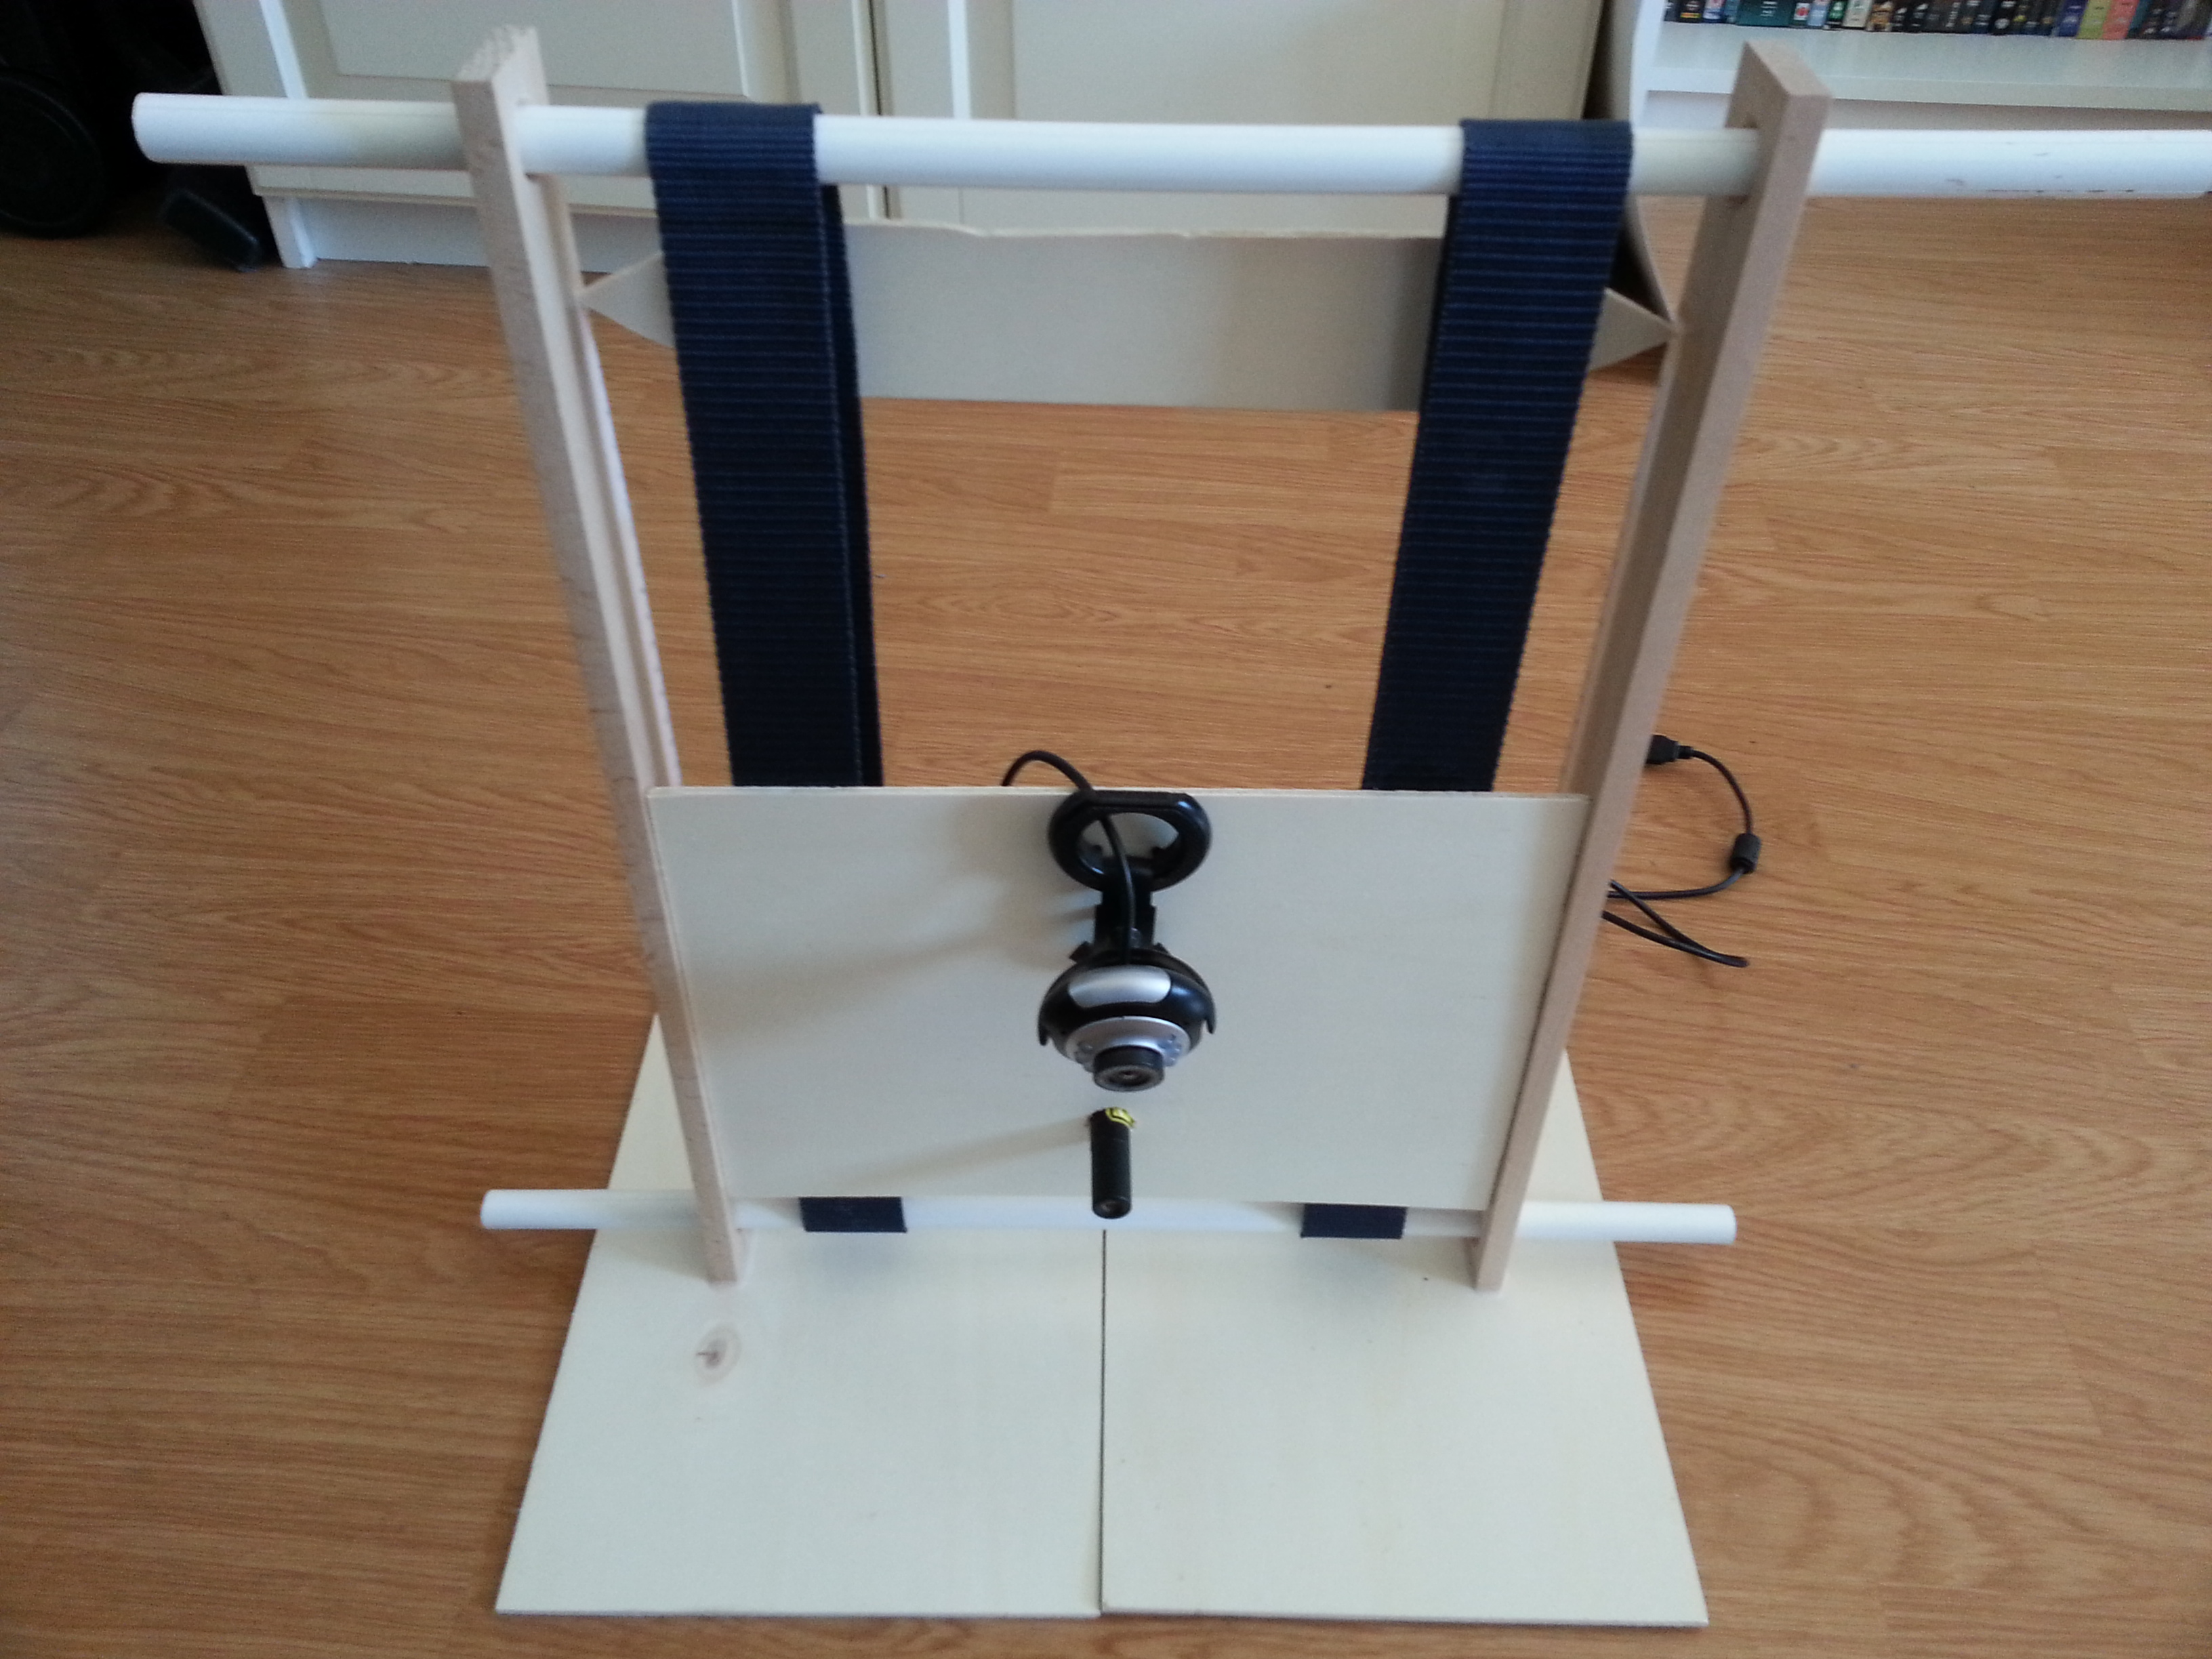
\includegraphics[width=\textwidth]{images/Scanner1.jpg}
\label{fig:scanner1}
\caption{Frontal Ansicht}
\end{minipage}
\begin{minipage}{0.45\textwidth}
\centering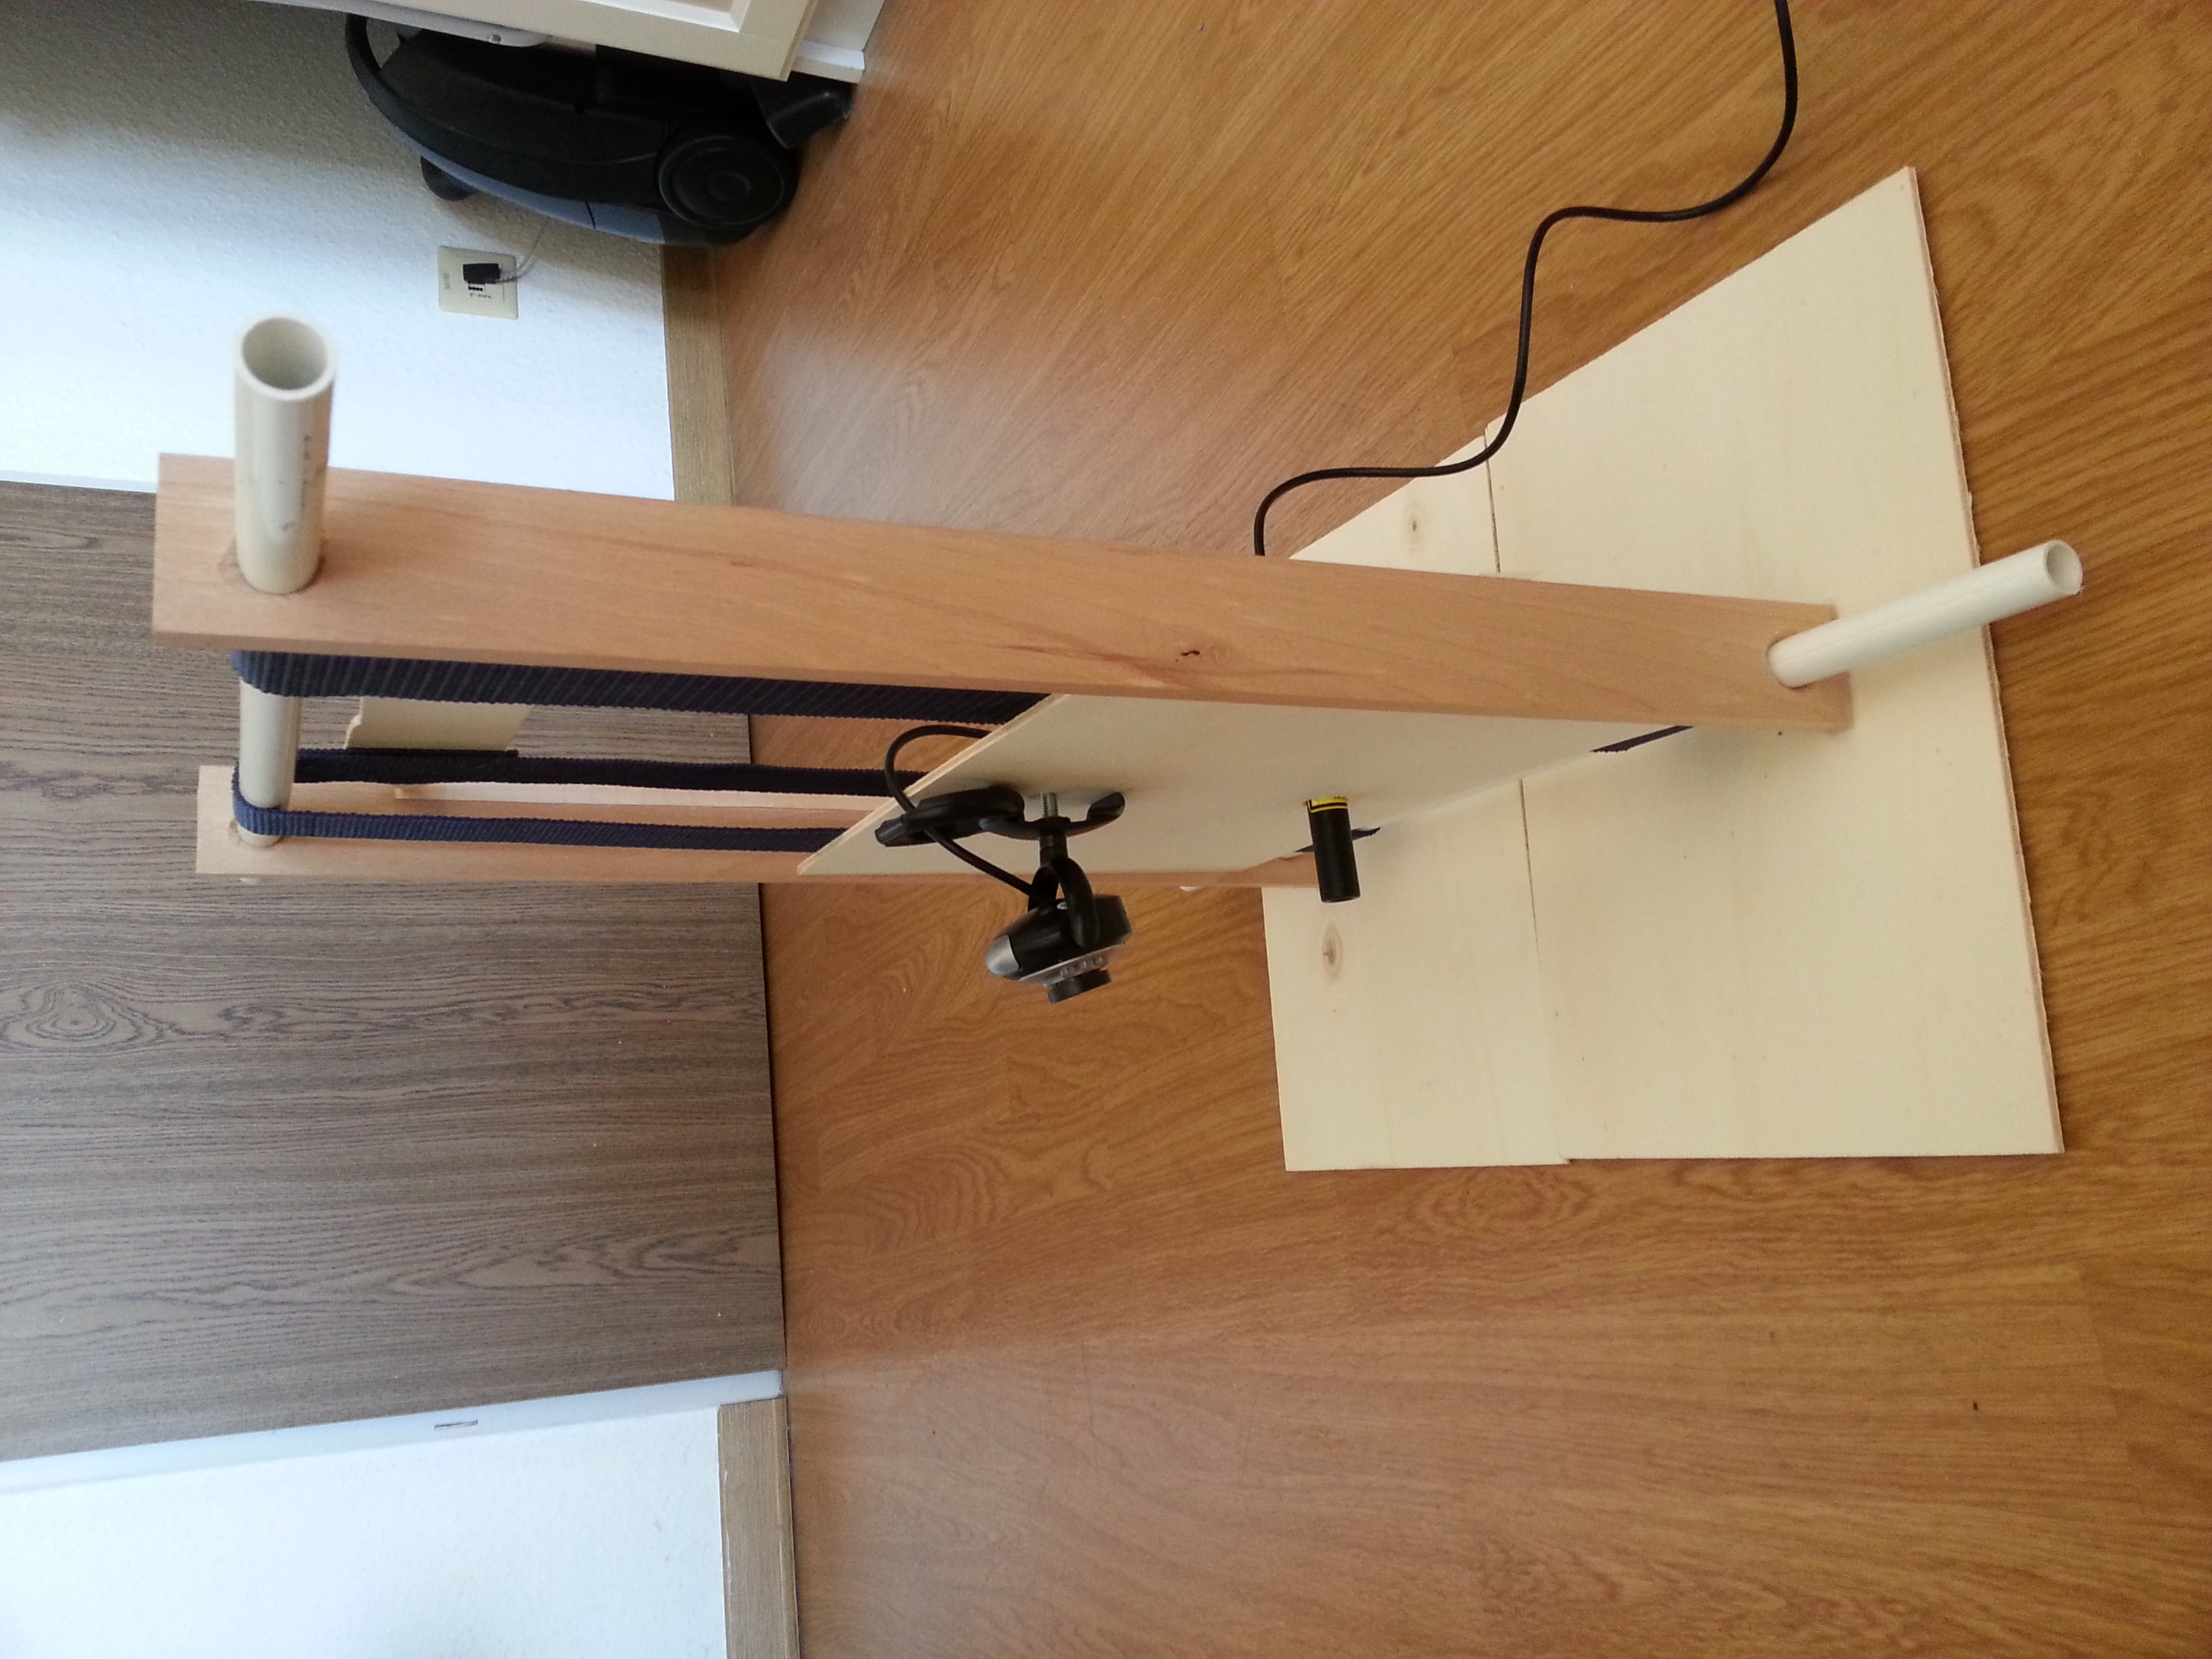
\includegraphics[width=\textwidth, angle = -90]{images/Scanner2.jpg}
\label{fig:scanner2}
\caption{Seitliche Ansicht}
\end{minipage}
\end{figure}

\begin{figure}
\centering 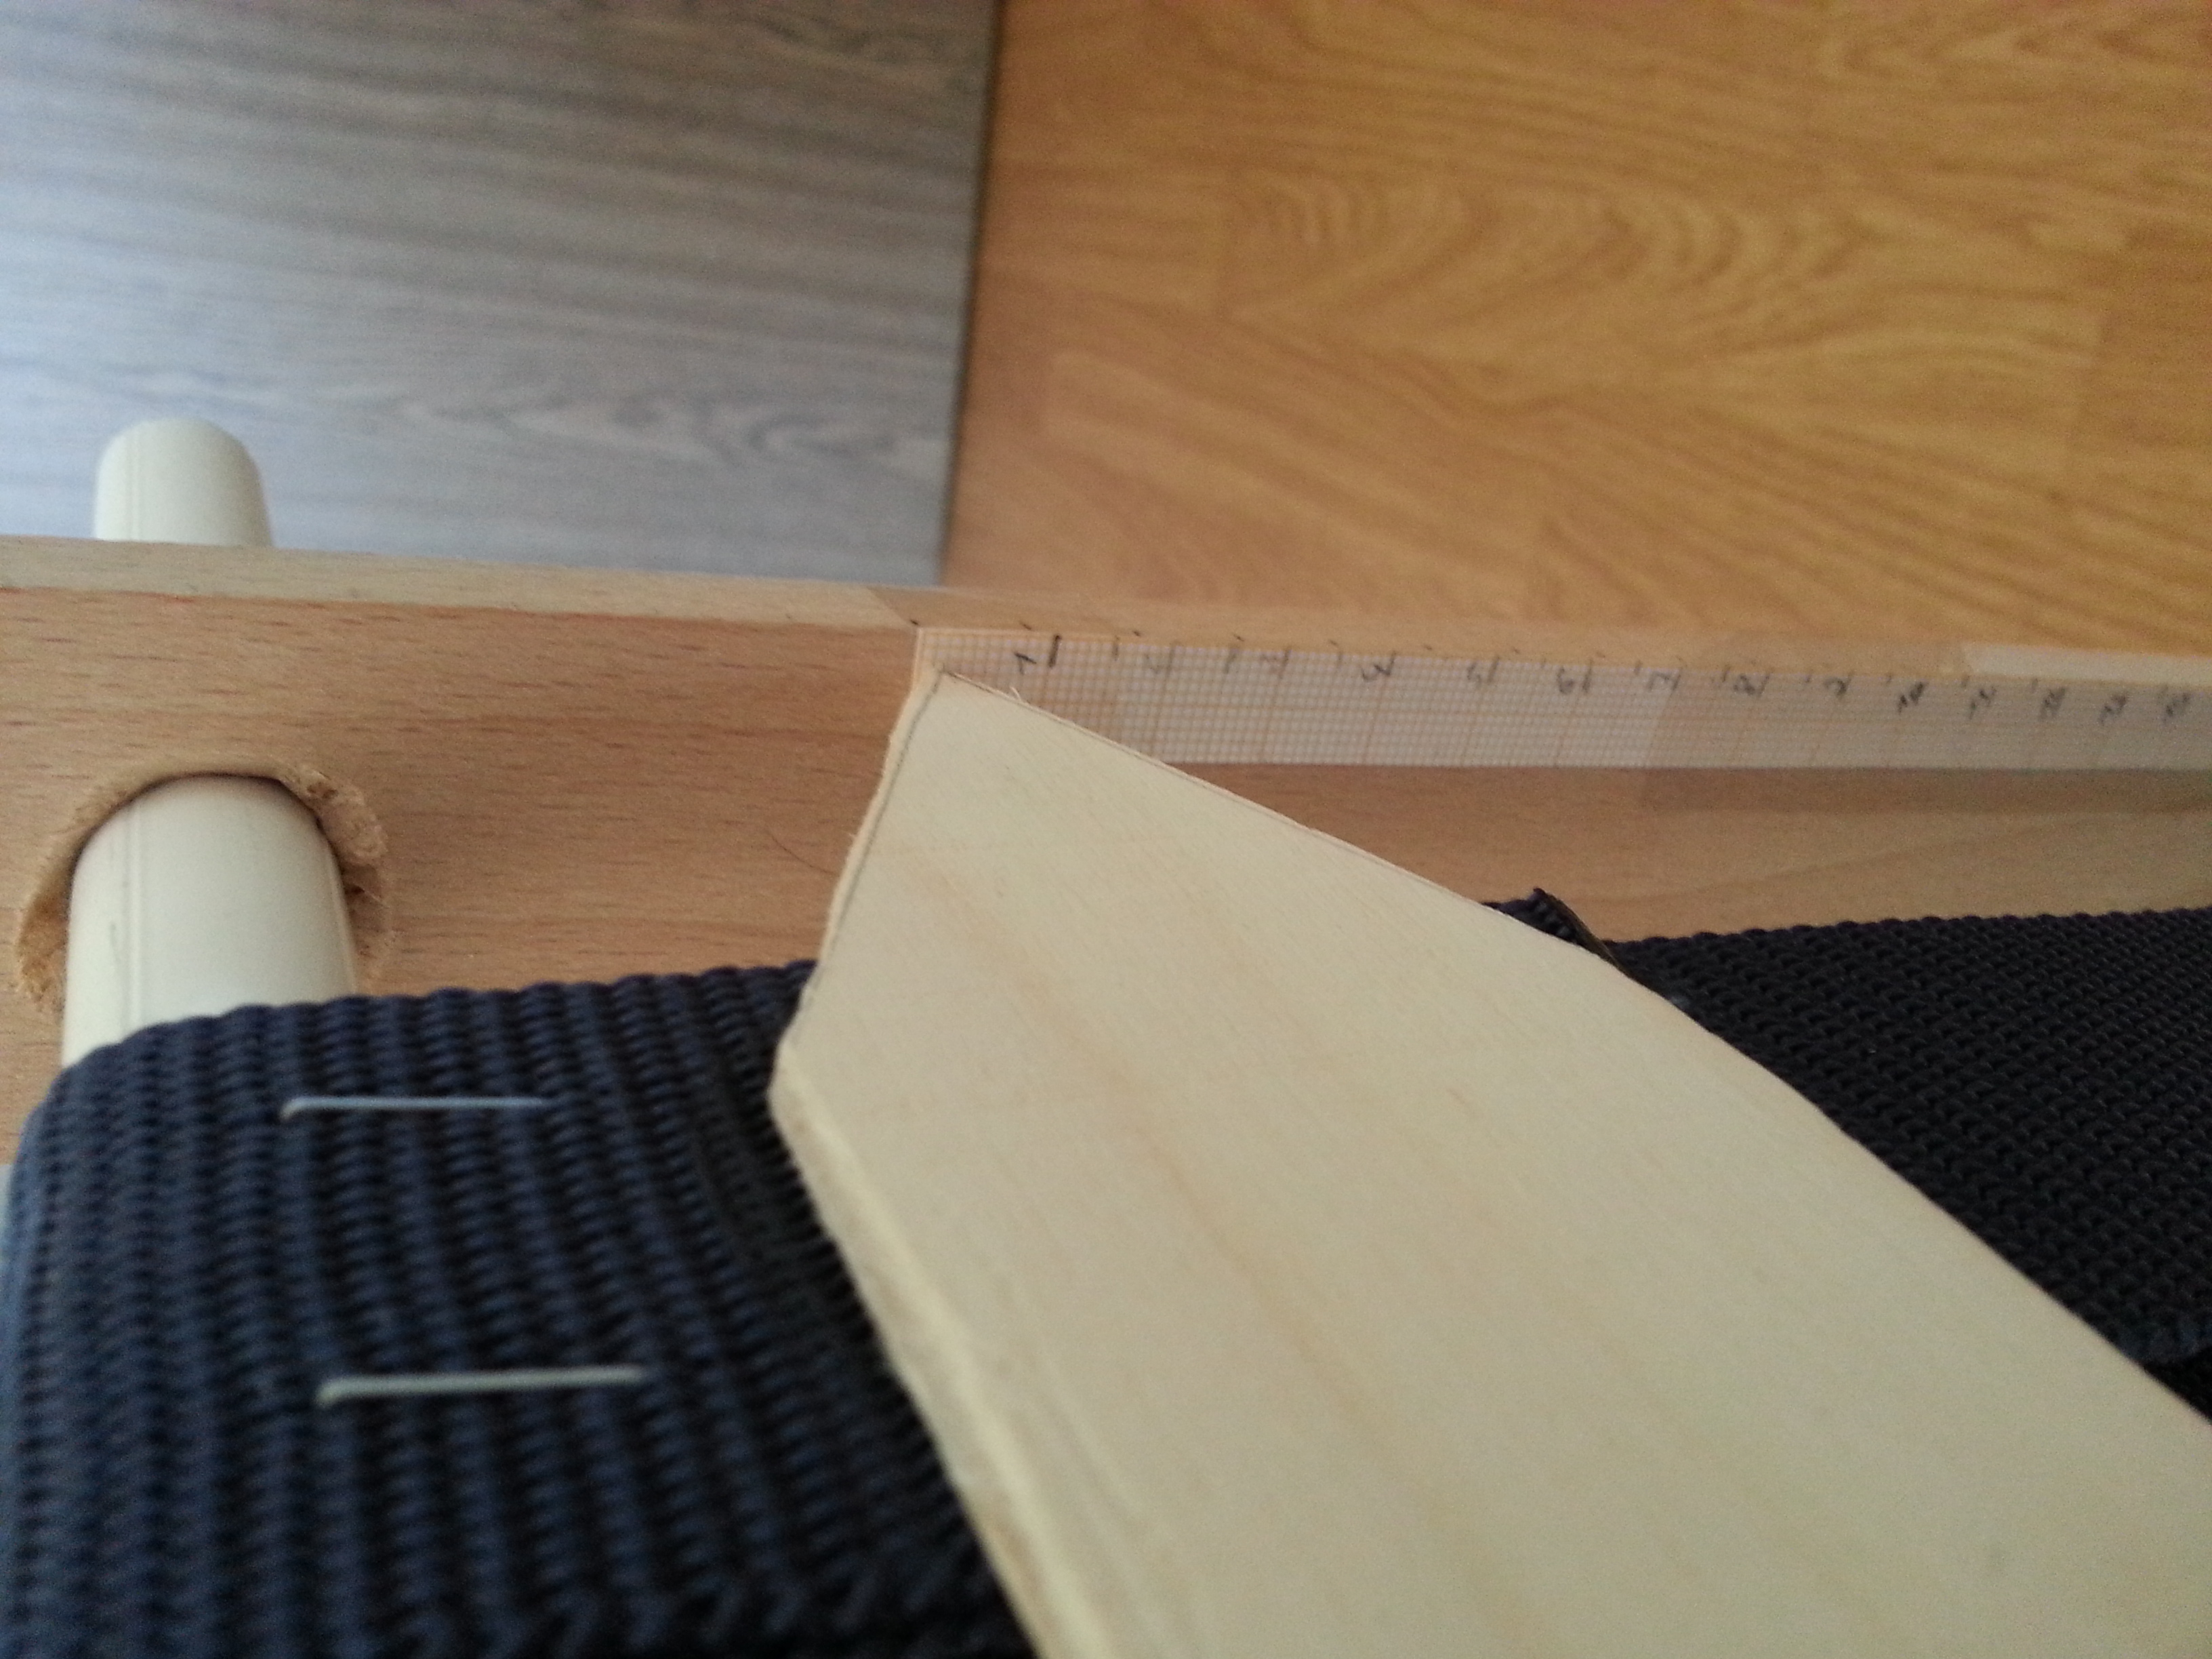
\includegraphics[width=0.5\textwidth, angle = -90]{images/Scanner3.jpg}
\label{fig:scanner3}
\caption{Nahaufnahme der Millimeter-Anzeige}
\end{figure}

Die vom Laser aufgespannte Ebene befindet sich somit parallel zum Grund, während die Kamera schräg von oben auf das zu vermessene Objekt schaut. Mittels des Gurts kann die Holzplatte, auf der Kamera und Laser montiert sind, von unten nach oben bewegt werden, um das Objekt so abzutasten. Um zu kontrollieren, wie weit der Laser über das Objekt bewegt wurde, ist auf der Rückseite des Gurts eine Anzeige installiert, welche sich gen Boden bewegt sobald Laser und Kamera nach oben steigen. Die Anzeige zeigt an den Seiten der Holzstreben, an denen eine Skala in Millieter-Papier angebracht ist, wie weit sich die Holzplatte von der Startposition aus nach oben bewegt hat. In Abb. \ref{fig:scanner3} ist eine Nahaufnahme dieser Anzeige zu sehen.

Ein wesentlicher Vorteil der vorgenommenen Konstruktion liegt in der Parallelität der Laser-Ebene zum Boden. Auf diese Weise muss man sich bei der späteren Bildverarbeitung keine Sorgen machen, dass die Laser-Linie auf den Untergrund fällt, auf dem das zu vermessene Objekt ruht. Wäre dies der Fall, müssten bei der späteren Auslesung die Teile der Laser-Linie, die auf das Objekt fallen, von denen, die auf den Untergrund fallen, aufwendig getrennt werden. Ebenfalls macht der Aufbau die Nachbearbeitung der gemessenen Weltkoordinaten im Gegensatz zu vergleichbaren Konstruktionen (z.B. bei schwenkbaren Scannern) besonders simpel: Da sich die Apparatur zwischen Aufnahmen lediglich entlang der Z-Achse bewegt und dieser Abstand bekannt ist, kann auf den Z-Achsen-Anteil des Messungsendergebnis der besagte Abstand einfach addiert werden.

Der Gesamtaufbau setzt vor allem auf eine praktikable Lösung, die problemlos nachgebaut werden kann und sich dem zu Grunde liegenden Problem so nähert, dass anschließende Verarbeitungen und Berechnungen erleichtert werden. Zudem ist die Konstruktion kostengünstig. In Tabelle \ref{tab:preise} können die Preise in Euro eingesehen werden, die alle Komponenten (außer Kleinteile wie einzelne Schrauben, Holzleim etc.) gekostet haben. Zusammen kommt der Scanner auf einen Preis von ca. 45,14\euro

\begin{table} %[hbtp]
	\centering
		\begin{tabular}{l | l}
		\textbf{Komponente} & \textbf{Preis in Euro}\\
		\hline
			Kamera "`TeckNet C016 USB HD Webcam"' & 13,99 \euro\\
			Linienlaser &  ca. 20 \euro\\
			PVC-Röhre & 1,69 \euro\\
			Holzleiste Buche (Seitenstreben) & 3,79 \euro\\
			Pappel-Sperrholz &  2,29 \euro\\
			Gurtband & 3,38 \euro
		\end{tabular}
	\caption{Bezeichnung der Tabelle}
	\label{tab:preise}
\end{table}


\section{Der Scanvorgang}
\label{sec:scanvorgang}
Um ein zu vermessendes Objekt in eine Reihe von abgetasteten Weltkoordinaten umzuwandeln wird in der vorliegenden Implementierung ein Prozess von verschiedenen Stufen vorgeschlagen. Der Gesamtprozess ist schematisch in Abb. \ref{fig:scanVorgang} dargestellt. Die einzelnen Stufen des Prozesses sind dabei nach der Abhängigkeit ihrer Ergebnisse und daraus folgen der Anzahl an nötigen Wiederholungen sortiert. Mit anderen Worten: Die Aktionen, die nur nur einmal ausgeführt werden müssen um mehrere Scanvorgänge zu ausführen zu können werden zuerst vorgenommen, während Aktionen die beispielsweise pro aufgenommenen Bild ausgeführt werden müssen, am Schluss folgen. Dies ist für denjenigen, der den Scanvorgang durchführt, eine geeignete Reihenfolge, da so Teilergebnisse für mehrere Scanprozesse wiederverwendet werden können und bei erfolglosen Stufen der Gesamtprozess nicht von neu angestoßen werden muss. \newline
Die Kalibrierung der internen Kameraparameter beispielsweise ist unabhängig von den anderen Umständen des eigentlichen Scanvorgangs und muss nicht für jede Messreihe erneut stattfinden, sondern lediglich wenn sich die Fokus-Einstellung der Kamera ändert. In der darauf folgenden Stufe des Scannens werden die nötigen Fotografien aufgenommen, was im Folgenden als Datenerhebung bezeichnet wird. Anschließend werden anhand einiger weniger dieser Bilder weitere Kalibrierungen vorgenommen, welche allerdings für den Rest des Datensatzes persistent sind und nur von Scandurchlauf zu Scandurchlauf wiederholt werden müssen. Zuletzt werden auf allen Bildern des Datensatzes die beiden Schritte der Laserlinienerkennung und Weltkoordinatenberechnung ausgeführt, welche für jedes Bild des Datensatzes andere Ergebnisse liefern und damit am Ende der Pipeline stehen. Die Weltkoordinaten, die als Resultat eines jeden Bildes berechnet werden, werden gesammelt und stehen als Punkte-Wolke zu weiteren Verarbeitung zur Verfügung. Im Folgenden werden nun die einzelnen Stufen des Scanvorgangs einzeln näher erläutert.


\begin{wrapfigure}{L}{0.45\textwidth}
\centering 
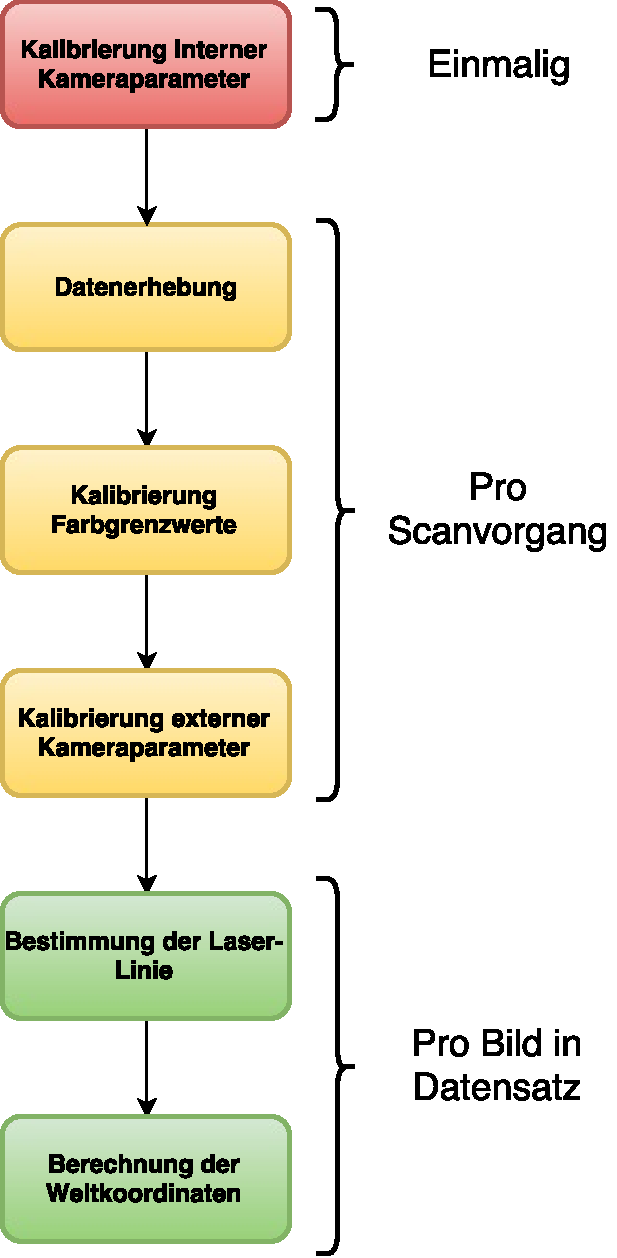
\includegraphics[width=0.45\textwidth]{images/ScannerVerfahren.pdf}
\label{fig:scanVorgang}
\caption{Der schematische Ablauf des Scanvorgangs}
\end{wrapfigure}
\leavevmode

\subsection{Kalibrierung der internen Kameraparameter}
In Abschnitt \ref{subsec:KameraKalibrierungTheorie} wurde die Theorie hinter der Kamerakalibrierung bereits erläutert, daher soll das Verfahren an dieser Stelle lediglich aus praktischer Sicht betrachtet werden. Aus Gründen, welche in \ref{fig:scanVorgang} dargelegt wurden, ist der Kamerakalibreirungsprozess in zwei zeitlich voneinander getrennte Teile gespalten. Am Anfang steht hierbei die Bestimmung der internen Kameraparamtern, insbesondere der internen Kameramatrix. Um diese abzuschätzen wurde auf die in Matlab integrierte Kamerakalibrirungsapp zurückgegriffen, welche aus einem Set von vorher aufgenommenen Bildern die Kameraparameter (wie in \ref{subsec:KameraKalibrierungTheorie} beschrieben) schätzt. Dabei werden eine Reihe von Kalibrierungsbilder, welche vorher aufgenommen wurden, in die App importiert und anschließend von jener verarbeitet. Bevor die nun geschätzte interne Kameramatrix als eigenständige Datei exportiert werden kann, sollten die sogenannten Reprojection Errors begutachtet werden. Diese stellen eine Metrik dar, welche besagt wie erfolgreich die Kalibrierung verlaufen ist und ergibt sich aus dem Abstand zwischen den im Bild erkannten Schachbrett-Punkten und den auf das Bild zurück projizierten korrespondierenden Weltkoordinaten (mehr dazu auch bei !QUELLE! und !QUELLE!). Bei den dieser Ausarbeitung mitgelieferten Kalibrierungsbilder wurde ein durchschnittlicher Reprojection Error von !WERT! erreicht, jedoch gilt laut einer Faustregel aus !QUELLE! jeder durchschnittliche Fehler von unter einem Pixel als akzeptabel. Am Ende der Kalibrierung muss die interne Kameramatrix gespeichert und für die weiteren Schritte hinterlegt werden.  

\subsection{Datenerhebung}
In der Phase der Datenerhebung werden die Fotografien des zu vermessenen Objektes aufgenommen. Dabei kommt die Konstruktion zum Tragen die in Kapitel \ref{sec:scannerKonstruktion} erläutert wurde. Zuerst muss die Messplatte in ihre Startposition gebracht werden, das heißt die Millimeter-Anzeige muss einen Abstand von 0 Millimetern anzeigen (vgl. Abb. \ref{fig:scanner3}. Anschließend muss das Schachbrettmuster, das auch bei der Kalibrierung der internen Kameraparametern zum Einsatz kam, so platziert werden, dass zum einen die Kamera alle Quadrate des Musters erkennen kann und zum anderen das zu vermessene Objekt so aufgestellt werden kann, dass die Laserlinie auf die unterste Peripherie des Objektes projiziert werden kann, also da, wo die Messung beginnen soll. Aufgrund der Konstruktion des Scanners muss das Schachbrettmuster dafür auf einer Erhöhung von ca. 9 cm ruhen. Für das erste Bild ist es jedoch wichtig, eine Aufnahme des Musters zu machen, auf dem das zu vermessene Objekt nicht abgebildet ist. Dieses Bild wird für die Kalibrierung der externen Kameraparameter benötigt, welche im kommenden Abschnitt \ref{subsec:externeKalibrierung} beschrieben ist. Von nun an ist es für den Rest des Scanvorgangs nicht mehr erlaubt, den Neigungswinkel der Kamera zu ändern.
Anschließend wird das zu vermessene Objekt so auf dem Schachbrettmuster platziert, dass die auf das Objekt projizierte Laserlinie in ihrer ganzen Länge zu erkennen ist und es wird eine Aufnahme gemacht. Nun muss die Messplatte mithilfe der Millimeter-Anzeige um einen vorher festgelegten Millimeter-Betrag nach oben bewegt werden. Der festgelegte Betrag muss für die spätere Berechnung der Weltkoordinaten festgehalten werden. Anschließend wird die nächste Fotografie geschossen. Dabei ist zu beachten, dass sich zwischen den Bildern nichts anderes als die Messplatte bewegen sollte und der vorher festgelegte Abstand so genau wie möglich eingehalten werden sollte. In dieser Manier wird nun das gesamte Objekt mit dem Laser abgetastet und je nach dem gewählten Abstand ergeben sich so mehr oder weniger Bilder, die für die folgenden Phasen abgespeichert werden.      

\subsection{Farbkalibrierung}
TODO

\subsection{Kalibrierung der externen Kameraparameter}
\label{subsec:externeKalibrierung}
TODO

\subsection{Bestimmung der Laserlinie}
TODO

\subsubsection{Berechnung der Weltkoordinaten}
\chapter{Ergebnisse}
Jedes Messverfahren muss sich vor allem durch seine Genauigkeit behaupten. Im folgenden Kapitel werden in dieser Hinsicht die Ergebnisse vorgestellt, die das in Kapitel \ref{chap:Implementierung} implementierte Verfahren erbracht hat. Dabei wird auch darauf eingegangen, warum die erläuterten Ansätze verfolgt wurden und inwiefern sie sich auf die Messergebnisse ausgewirkt haben. Für die folgenden Erklärungen wurde die ebenfalls vorliegende exemplarische Messreihe einer im Raum liegenden schiefen Ebene verwendet, welche sich aufgrund ihrer geometrisch einfachen Form leicht beschreiben und als Validierungsobjekt verwenden lässt.   

\section{Laserlinienbestimmung}
\label{subsec:segmentierung}

Die Lokalisierung der Laserlinie bestimmt in Bildkoordinaten, welche Teile des Bildes für die Messung interessant sind. Jegliche Ungenauigkeiten die in diesem Schritt auftreten propagieren sich also unweigerlich in den Folgeschritten zu immer größeren Messfehlern. Eine sorgfältige Bildverarbeitung ist hier also von hoher Bedeutung.\bigbreak
Wie in Abschnitt \ref{subsec:Farbkalibrierung} und \ref{subsec:LaserLinieBestimmung} beschrieben, wird für die Segmentierung der Laserlinie auf einen globalen Farbgrenzwert gesetzt. Dieser Ansatz erweist zwar eine geringe Komplexität, ist aber nicht ohne Nachteile. In \ref{fig:farbwerte} sind exemplarisch die Farbkanalwerte für die Pixel einer einzelnen Bildspalte aus einem ausgewählten Bild (welches in Abb. \ref{fig:LineDistanceSchematic} ganz oben zu sehen ist) sowohl im RGB- als auch im YCbCr-Farbraum dargestellt. Dabei befinden sich auf der X-Achse die Reihenindizes und auf der Y-Achse die Kanalwerte im Bereich von \(0\) bis \(255\). Wie man der Abbildung erkennen kann, befindet sich die Laserlinie im X-Achsenabschnitt ca. zwischen \(370\) bis \(380\), erkennbar durch den hohen Ausschlag im Rot-Kanal. Möchte man nun einen globalen Farbgrenzwert ansetzen um die Laserlinie in ihrer gesamten Breite von ca. \(10\) Pixel zu erfassen und dabei alle anderen Bildanteile auszublenden, müssten alle Pixel mit einem Rotkanalwert von unter \(80\) ausgeblendet (also geschwärzt) werden. Dabei bleiben aber noch die Pixel übrig, die sowohl einen hohen Rot- als auch einen hohen Blau und Grün-Anteil aufweisen und somit ebenfalls nicht zur Laserlinie gehören. Es würde sich nun also anbieten, für den Grün- und Blau-Kanal einen Obergrenzwert festzulegen, der zusätzlich alle Pixel schwärzt, deren Grün- und Blau-Anteile die über diesen Obergrenzwerten liegen. Wie aus Abb. \ref{fig:farbwerte} allerdings hervorgeht, ist es nicht möglich, solche Grenzwerte zu finden und gleichzeitig alle Pixel der Laserlinie zu erhalten. Vor allem im X-Achsenabschnitt von \(0\) bis \(150\) sind die Grünkanalwerte nicht hoch genug um durch die Obergrenze geschwärzt zu werden und gleichzeitig die Pixel im X-Achsenabschnitt von \(370\) bis \(380\) intakt zu lassen (ähnliches gilt für die Blau-Werte in anderen Teilen des Bildes). Eine Alternative bestünde darin, den Rotkanal-Untergrenzwert zu erhöhen, um die hohen Rotkanalwerte im X-Achsenabschnitt von \(0\) bis \(150\) auszublenden, was allerdings in einer generellen Schmälerung der Laserliniensegmentierung resultiert.\linebreak
In der vorliegenden Implementierung wurde nun anstatt eines RGB- ein YCbCr-Grenzwert verwendet. Dieser ist ebenfalls in Abb. \ref{fig:farbwerte} abgebildet. Das geschilderte Problem lässt sich zwar auch in diesem Farbraum nicht gänzlich vermeiden, jedoch besser kontrollieren. Indem nur ein Grenzwert angepasst werden muss, nämlich der Cr-Grenzwert, eignet sich dieser Farbraum zur besseren automatischen Grenzwertfindung, welche sicherstellen soll, dass die Schmälerung der Laserliniensegmentierung minimal ausfällt.   
\bigbreak
Ohne eine lokale Betrachtung der Bilddaten lässt sich mit einem globalen Ansatz die Segmentierung der Laserlinie also nicht zur  Gänze beseitigen. Daher wird in der vorliegenden Implementierung wie in \ref{subsec:LaserLinieBestimmung} beschrieben darauf gesetzt, nach einer groben Lokalisierung auf Basis der Segmentierung eine feinere Bestimmung auf Basis der umliegenden unsegmentierten Pixeldaten vorzunehmen. So wird der Nachteil eines globalen Farbgrenzwertes abgeschwächt ohne zu viel Komplexität hinzuzufügen. Die Ergebnisse der Laserlinienbestimmung bewegen sich dank dieses Ansatzes in einem akzeptablen Fehlerraum. In \ref{fig:LaserLinieExtraktion} ist eine mit dem Verfahren erkannte Laserlinie zu sehen, welche neben einem vom Benutzer vorgenommenen Goldstandard und vor dem Hintergrund des betreffenden Bildes dargestellt ist. Der Cr-Grenzwert der in diesem Beispiel gewählt wurde ist durch dass Verfahren ermittelt worden, welches in \ref{subsec:Farbkalibrierung} beschrieben wurde. Die Distanz zwischen der optimalen und der ermittelten Linie beträgt \(5.0443\) Pixel.

\begin{figure}
\centering \includegraphics[width=\textwidth]{images/Colour.pdf}
\caption[Farbkanäle einer einzelnen Bildspalte]{Farbkanäle einer einzelnen Bildspalte}\label{fig:farbwerte}
\end{figure}

\section{Messgenauigkeit}
Die Genauigkeit der Berechnung der Weltkoordinaten bestimmt wie erfolgreich das Messverfahren in seiner Gesamtheit funktioniert, da diese das angestrebte Endprodukt der Messung darstellen. Um diese Genauigkeit zu bestimmen, wurde für die vorliegende Implementierung die zu Eingang des Kapitels erwähnte schiefe Fläche zweimal vermessen: Einmal händisch um nötige Daten für die mathematische Beschreibung der Schräge zu sammeln, und einmal mit dem Lichtschnittverfahren um diese Messung mit der händischen Messung zu vergleichen. Durch die händische Messung lässt sich die Schräge mathematisch vergleichsweise einfach als eine durch vier Seiten begrenzte Ebene beschreiben und eignet sich daher zur Berechnung einer Metrik, mit der die Exaktheit des Verfahrens bewertet werden kann. Dafür wird für jede Weltkoordinate der kürzeste Abstand zur Ebene berechnet. Es wird immer der kürzeste Abstand zum jeweils nächsten Merkmal der Schräge ermittelt, also entweder zur Ebene an sich, zu einer der vier Seiten oder einer der vier Eckpunkte der Fläche. Anschließend wird der Median dieser Abstände gebildet, um zu ermitteln, wie weit eine Koordinate im Durchschnitt von der eigentlichen Fläche entfernt ist. In \ref{fig:MessungSlope} ist die gemessene Punktewolke der eigentlichen Schräge entgegengestellt. Gemessen wurden hier \(2168\) Punkte, welche im Durchschnitt \(0.9083\)mm mit einer Standardabweichung \(\sigma = 0.5360\) von  der optimalen Schräge entfernt liegen. \bigbreak

\begin{figure}
\centering 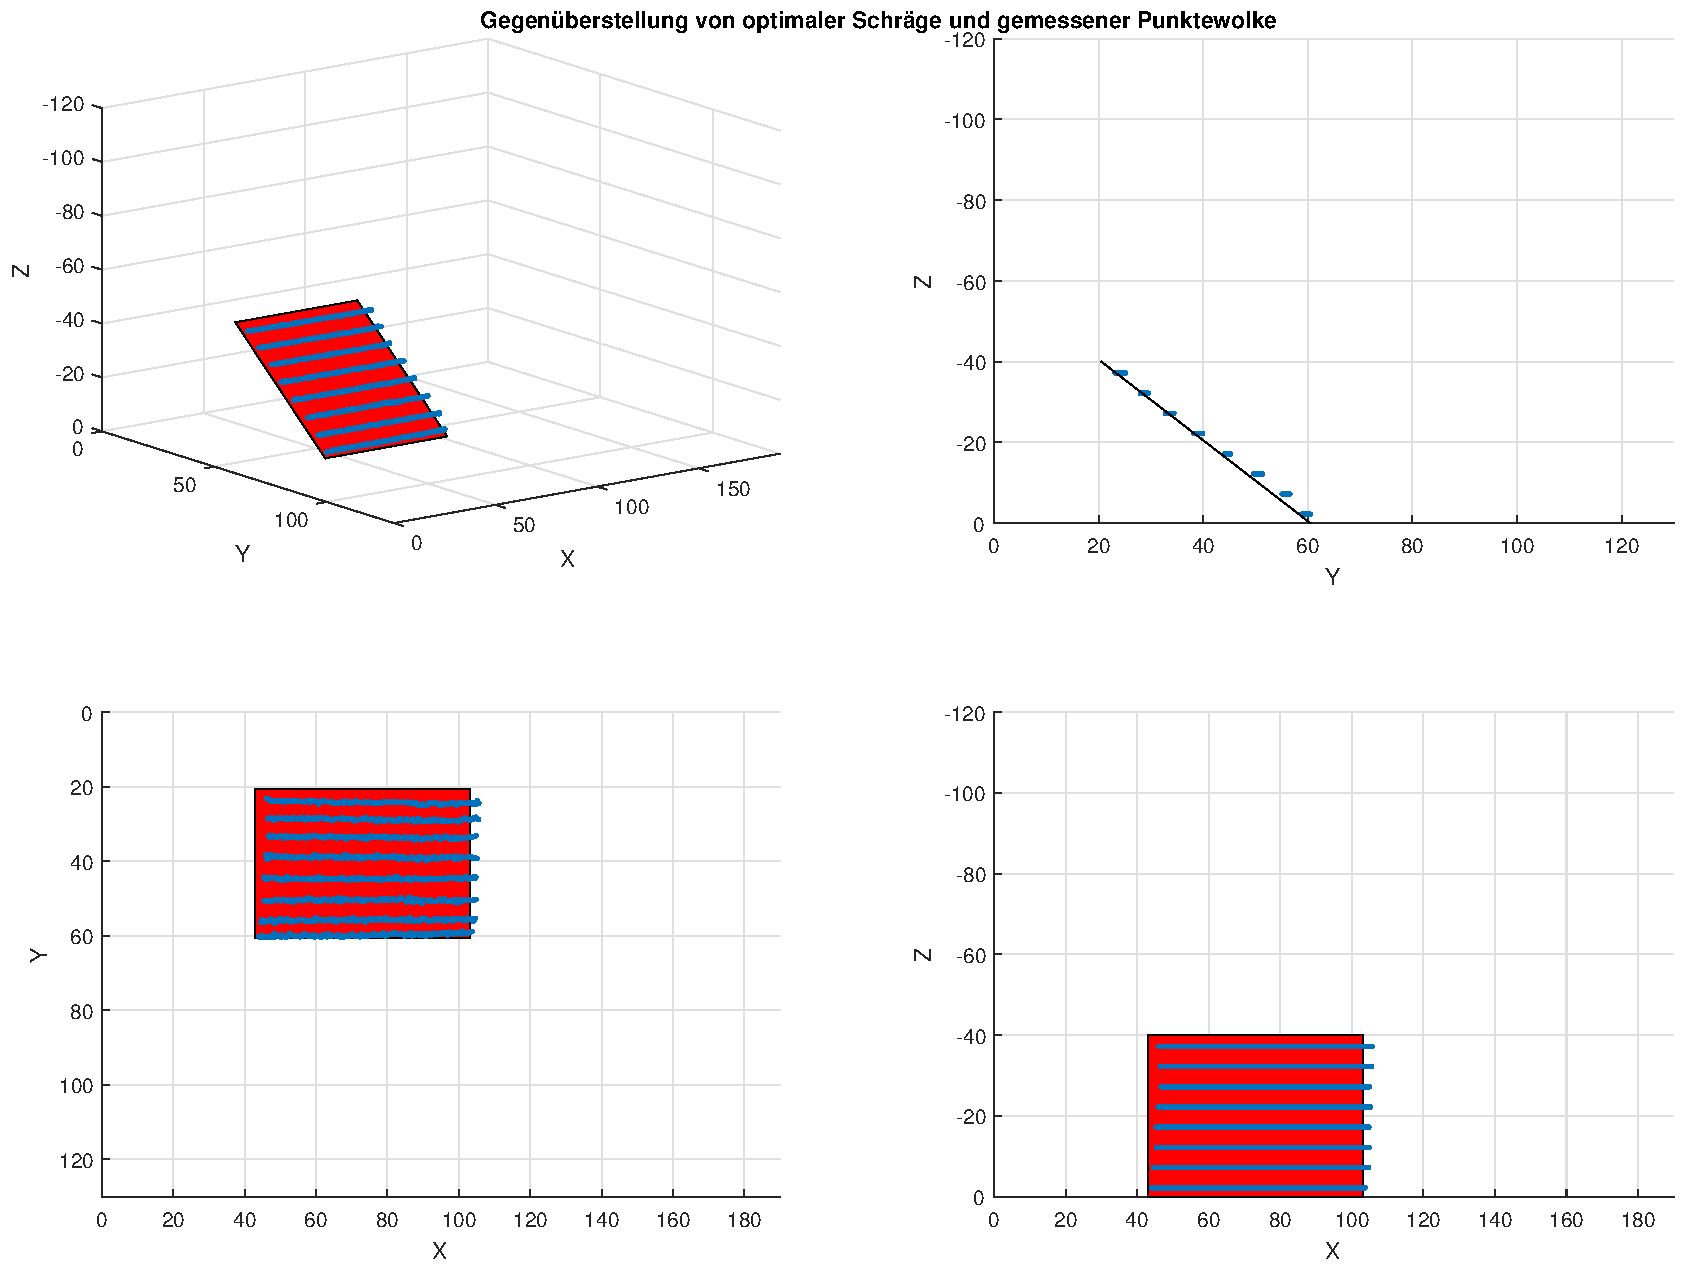
\includegraphics[width=\textwidth]{images/Messung.pdf}
\caption[Gegenüberstellung von optimaler Schräge und gemessener Punktewolke]{Gegenüberstellung von optimaler Schräge und gemessener Punktewolke}\label{fig:MessungSlope}
\end{figure}

In Abb. \ref{fig:MessungSlope} ist auf der X-Y-Ebene zu sehen, dass die einzelnen vermessenen Punkte-Linien eine Schiefe aufweisen und nicht im perfekten rechten Winkel zu X-Achse stehen. Dies ist der Tatsache geschuldet, dass der Laser während der Bildaufnahmen nicht ganz parallel zur Bodenebene stand. Als Resultat neigt sich auch auf den Bildern die Laserlinie mit einer leichten Steigung, was den oben zu sehenden Effekt hervorbringt. Dies lässt sich vor allem mit erhöhter Sorgfalt während des Vermessens mildern, zeigt jedoch, dass Außeneinflüsse im direkten Vergleich zu mathematisch optimalen Kontrukten selten zur Gänze zu vermeiden sind.\linebreak
Ein Problem des Verfahrens liegt ebenfalls in der Gefahr, dass die mathematische Beschreibung des Validierungsobjektes das Objekt idealer beschreibt als in der Realität abgebildet. Somit kann die Messung zu einem gewissen Grad niemals an die mathematische Beschreibung heran reichen und der Messung wird auf diese Weise "Unrecht getan", also schlechter eingeschätzt als sie eigentlich ist. Dennoch kann bei genügender Sorgfalt der händischen Vermessung des Objektes damit gerechnet werden, dass die Metrik aussagekräftig ist. Auch wenn die verwendete Metrik nur für das simple Validierungsobjekte sprechen kann, wird davon ausgegangen dass sich das implementierte Verfahren für komplexere Objekte ähnlich genau verhält.
\chapter{Fazit}
Der Laserscanner, der für die vorliegend implementiert wurde, erfüllt seine Funktion zuverlässig: Innerhalb von wenigen Schritten kann ein Objekt abgetastet und mit einem vertretbaren Messfehler als dreidimensionale Punktewolke dargestellt werden. Auch bei weniger simplen Objekten kann so ein Modell erstellt werden, welches die Charakteristika des Gegenstandes in wiedererkennbarer Weise zuverlässig darstellt. In !BILD! sieht man beispielsweise eine Messung einer kleinen Statuette, welche einem Foto des originalen Objektes gegenübergestellt ist. Das Objekt lässt eindeutig wiedererkennen. Der nächste natürliche Schritt in der Verarbeitungspipeline wäre nun die Triangulation der Punktewolke um ein zusammenhängendes Mesh zu erhalten. Dies ist jedoch außerhalb des Zu\-stän\-dig\-keits\-bereichs der vorliegenden Ausarbeitung.\newline
Einige Verbesserung wären für eine Verfeinerung des Verfahrens jedoch durchaus denkbar. Zum Einen bietet die Scannerkonstruktion an sich Raum für Verbesserung: Anstatt die gleichmäßige Abtastung der manuellen Einstellung zu überlassen, könnte ein Mechanismus ersannt werden, der es einfacher macht, den Abstand zwischen Aufnahmen genau einzuhalten. Ebenfalls wäre hier die Möglichkeit wünschenswert kleinere Abstände während der Messung einzuhalten um so eine größere Dichte der Punktewolke zu erhalten. Während eine vollständige Automatisierung hier die beste Lösung darstellt (jedoch den Preis des Laserscanners zugleich erhöhen würde), ist ein Mechanismus wie zum Beispiel eine mechanische Schraube zum Einstellen des Abstandes möglich. Eine andere Erweiterungsmöglichkeit der Scannerkonstruktion stellt die Unterstützung von Messungen von mehr als einer Seite des Objekts dar. Dies würde es möglich machen, das gesamte Objekt als Punktewolke abzubilden. Am Berechnungsanteil des Verfahrens sind alternative Vorgehensweisen an einigen Stellen denkbar. So könnte zum Beispiel bei der Laserlinienerkennung statt mit einem globalen mit einem adaptiven Schwellwert gearbeitet werden, was zwar zu Lasten der Komplexität des Algorithmus' gehen würd, aber gegebenenfalls gute Ergebnisse liefern könnte. \newline
Auch bei verbleibendem Potential für Verbesserung bietet der implementierte Scanner eine solide Basis zur weiteren Verfeinerung und erfüllt seine Designziele angemessen. Er erlaubt zuverlässige Messungen und demonstriert das Lichtschnittverfahren auf eine praktikable Art und Weise. 
% ...
%--------------------------------------------------------------------------
\backmatter                        		% Anhang
%-------------------------------------------------------------------------
%\bibliographystyle{geralpha}			% Literaturverzeichnis
%\bibliography{literatur}     			% BibTeX-File literatur.bib
%--------------------------------------------------------------------------
\printindex 							% Index (optional)
%--------------------------------------------------------------------------
%\begin{appendix}						% Anhänge sind i.d.R. optional
%   \include{chapters/Glossar}			% Glossar   
%   \chapter{Erkl�rung der Kandidatin / des Kandidaten}

\begin{description}[$\Box$~]
\item[$\Box$] Die Arbeit habe ich selbstst�ndig verfasst und keine anderen als die angegebenen Quellen- und Hilfsmittel verwendet.\\

\item[$\Box$] Die Arbeit wurde als Gruppenarbeit angefertigt. Meine eigene Leistung ist\\
...\\

Diesen Teil habe ich selbstst�ndig verfasst und keine anderen als die angegebenen Quellen und Hilfsmittel verwendet. \\

Namen der Mitverfasser: ...

\end{description}

\vspace{2cm}

\begin{minipage}[t]{3cm}
\rule{3cm}{0.5pt}
Datum
\end{minipage}
\hfill
\begin{minipage}[t]{9cm}
\rule{9cm}{0.5pt}
Unterschrift der Kandidatin / des Kandidaten
\end{minipage}	% Selbstständigkeitserklärung
%\end{appendix}

\end{document}
